\documentclass[12pt]{article}
\usepackage{parskip}
\usepackage{amsmath}
\usepackage{pdfpages}
\usepackage{listings}
\usepackage{color}
\usepackage[margin=.6in]{geometry}

\definecolor{dkgreen}{rgb}{0,0.6,0}
\definecolor{gray}{rgb}{0.5,0.5,0.5}
\definecolor{mauve}{rgb}{0.58,0,0.82}

\lstset{frame=tb,
  language=C++,
  aboveskip=3mm,
  belowskip=3mm,
  showstringspaces=false,
  columns=flexible,
  basicstyle={\small\ttfamily},
  numbers=none,
  numberstyle=\tiny\color{gray},
  keywordstyle=\color{blue},
  commentstyle=\color{dkgreen},
  stringstyle=\color{mauve},
  breaklines=true,
  breakatwhitespace=true,
  tabsize=3
}

\begin{document}
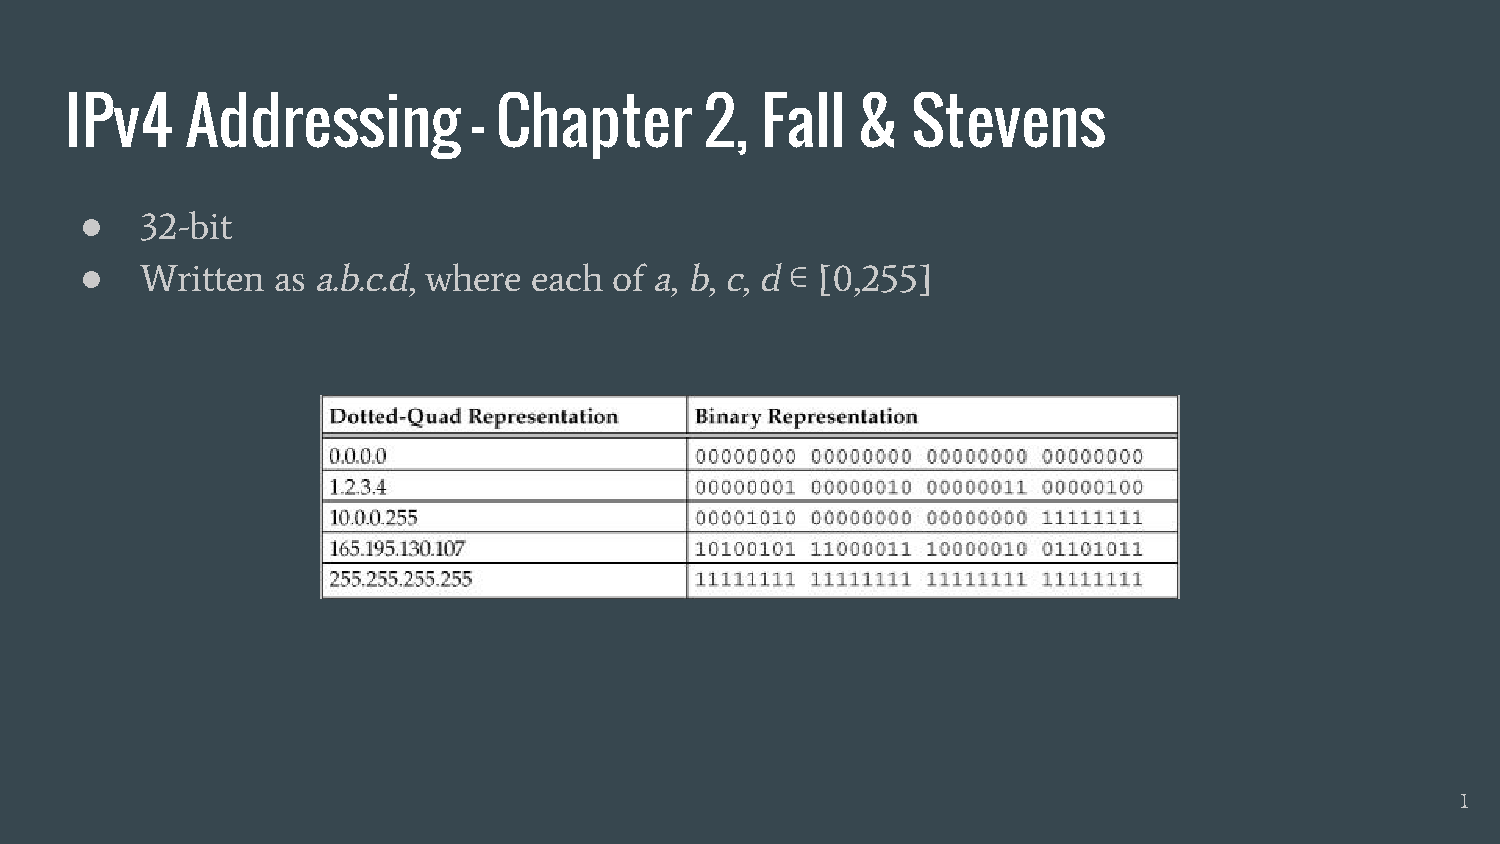
\includepdf[page=1-2]{slides.pdf}
Originally there was just some bits allocated to the network and some bits allocated to the hosts. The leading bits are used to determine what class of address it is. 

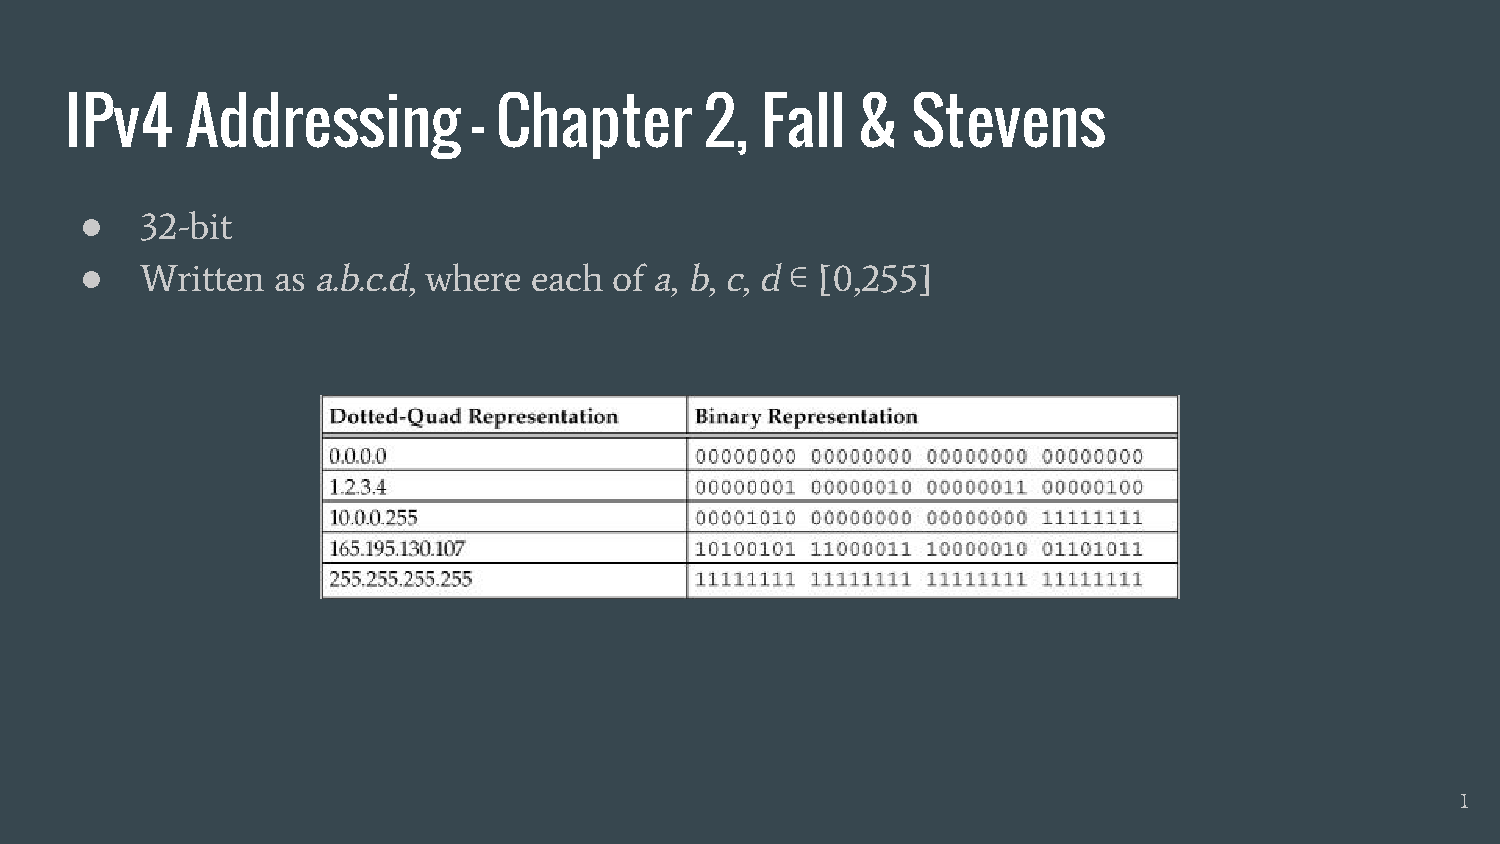
\includepdf[page=3]{slides.pdf}
When you are working with class B addresses you can steal some bits from the hosts to have a subnet.

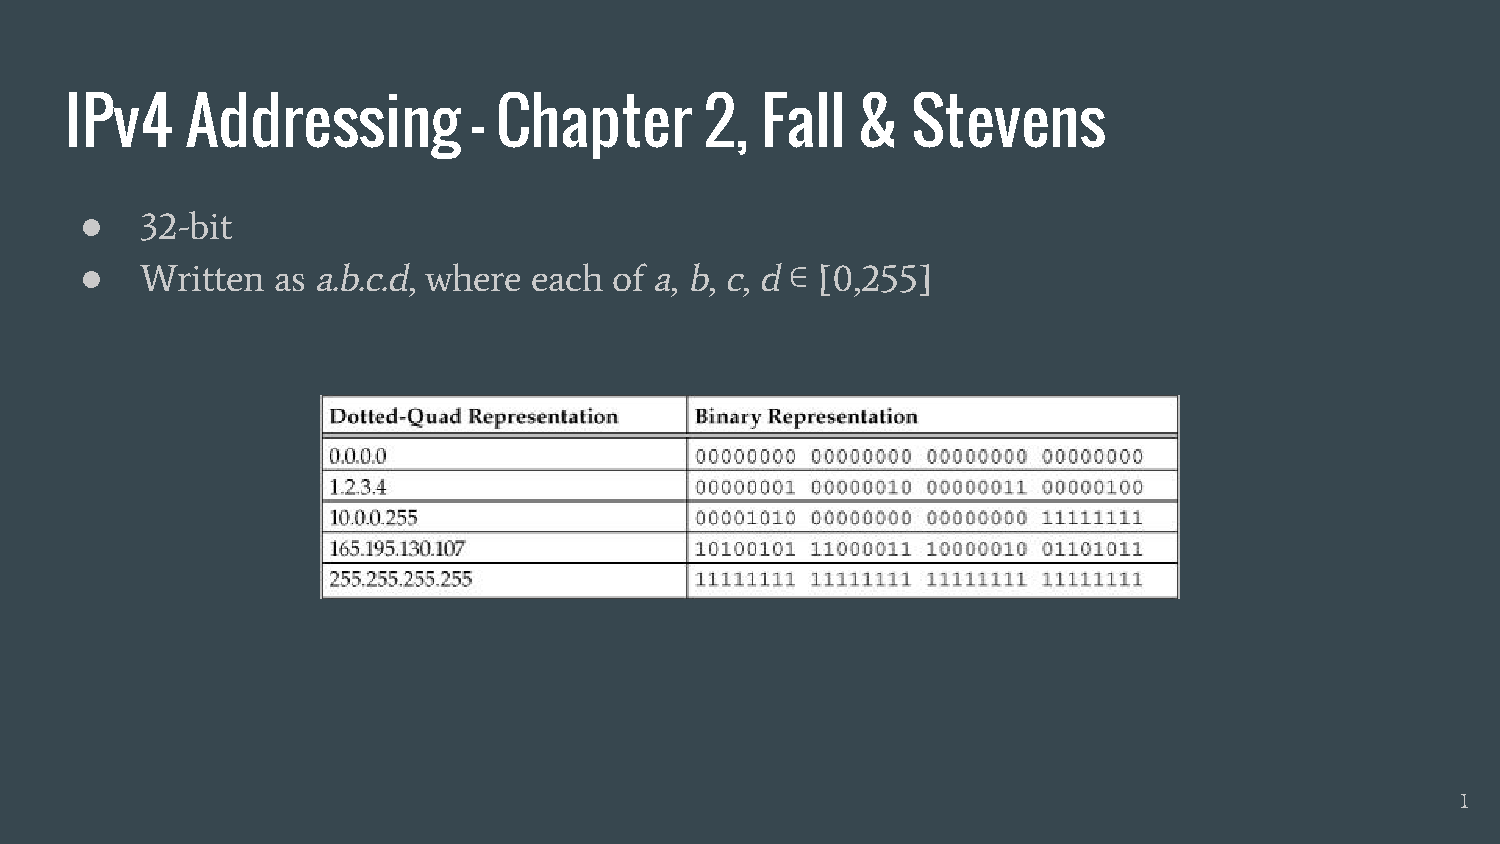
\includepdf[page=4]{slides.pdf}
We can apply a mask to an ipaddress by doing a bitwise and to get prefixes. It can be denoted by /# where the number is the number of 1s in the mask. So 1.1.0.0/16 tells us we only care about the first 16 bits of the address.

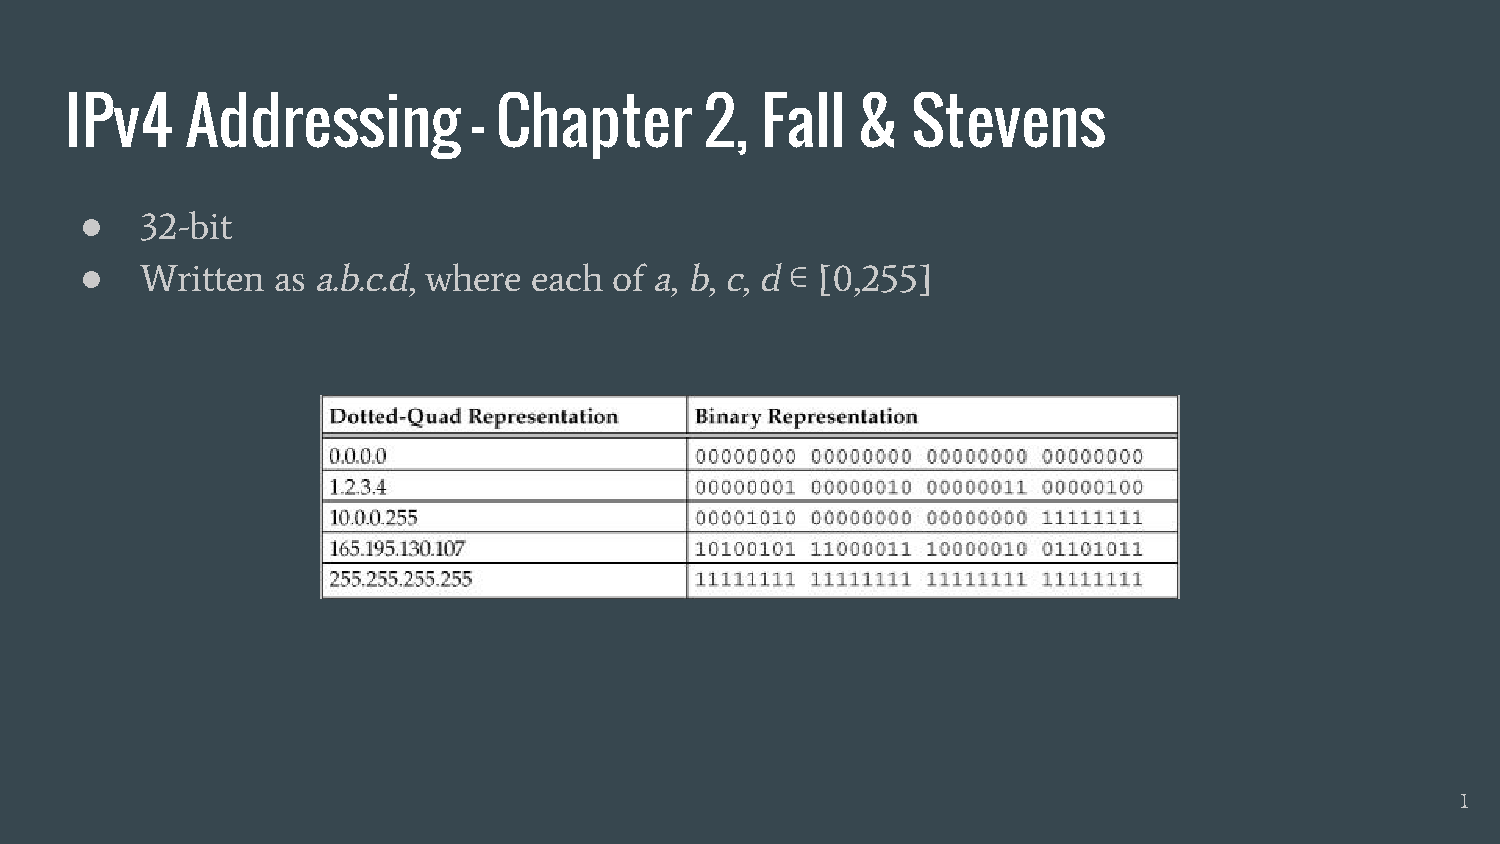
\includepdf[page=5]{slides.pdf}
We can see they they have a class B (since 128 is 10000000) with two hosts. Their router has to properly route to those two, it must use a mask to do so. Anything that you have to do with software in a network is bad (mainly for performance reasons). With a routing table we have just the destination address (we dont give a shit about the content). Masks make this harder because they have a concrete destination address and match it against a network prefix. There is no good way to do this. What we do is take the network prefix out and see how many destinations there could be and enumerate the possibilities in a table. This makes the lookup ridiculously fast but uses a bunch of memory. The memory is called TCAM which directly influences your speed but is super expensive. 

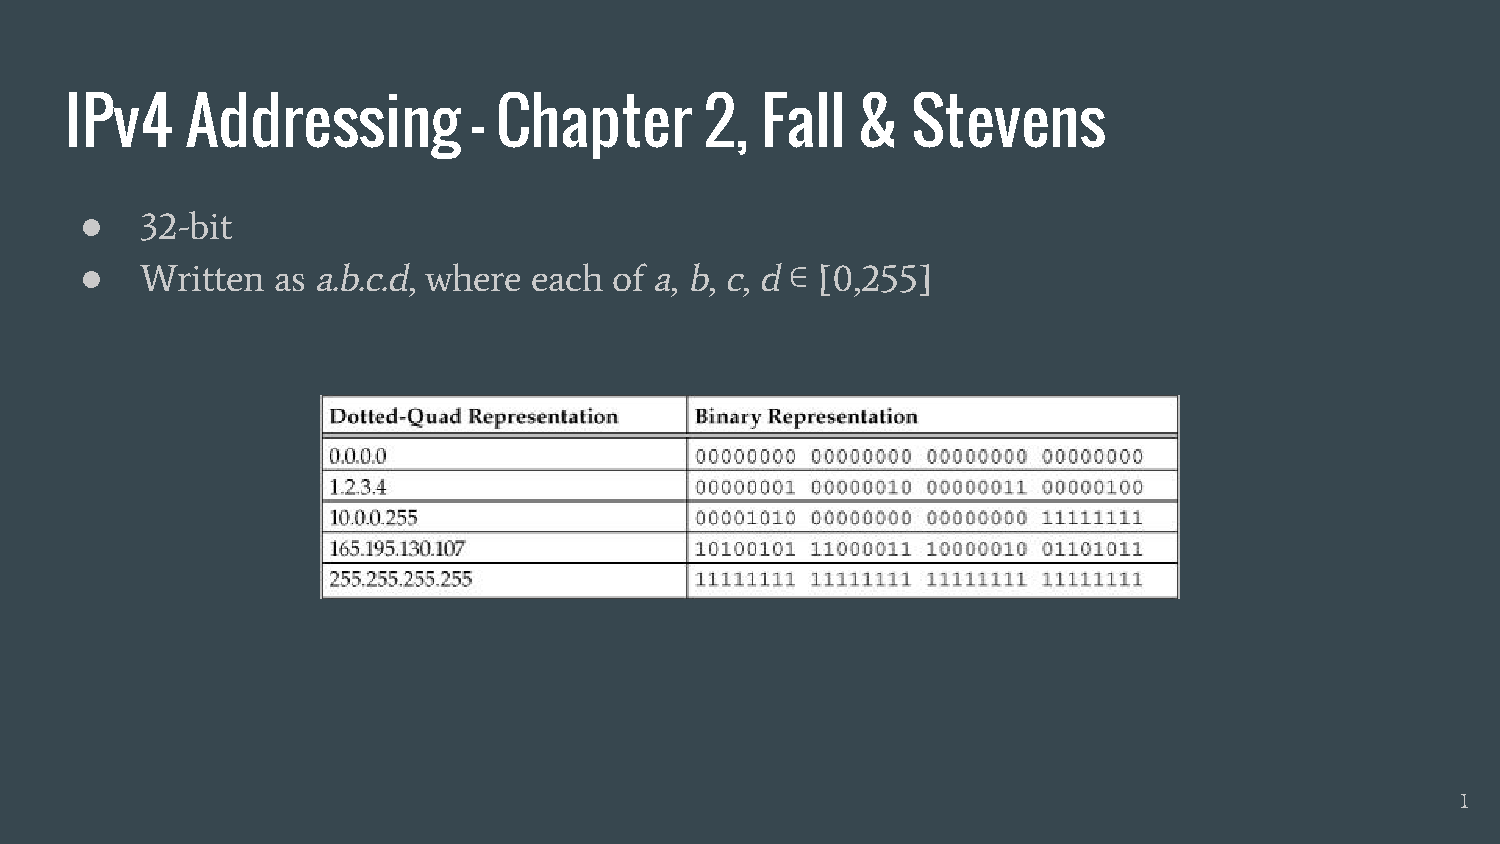
\includepdf[page=6]{slides.pdf}
Say we have a prefix of length 24. When you do the bitwise and you get then network id. Just do this example. 

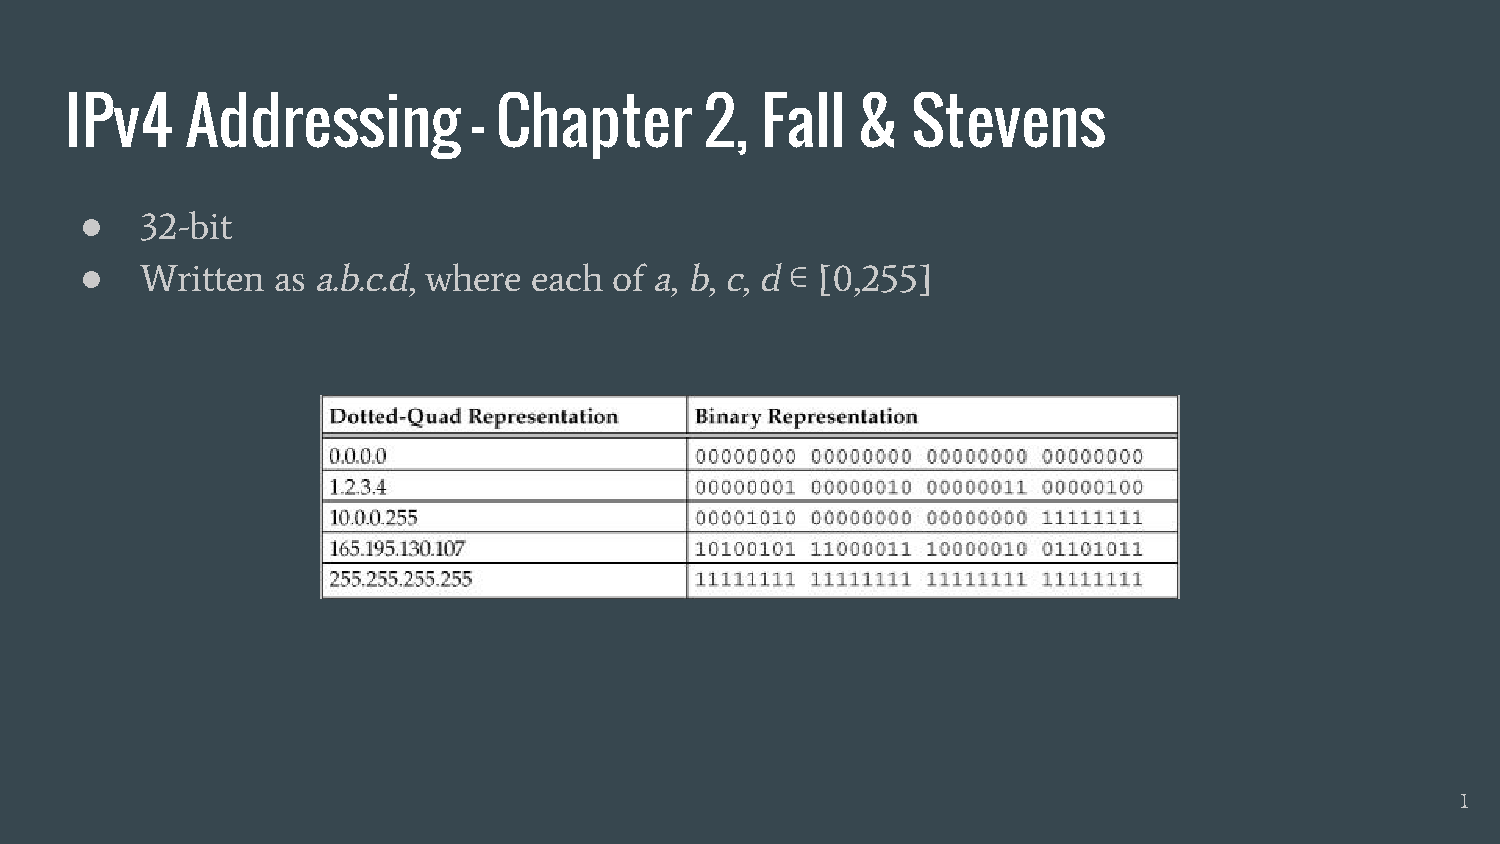
\includepdf[page=7]{slides.pdf}/
What if we want subnets to be different sizes. We want to make the most use of our ipaddresses since they are valuable resources. We can do this by having variable network prefixes. You have to be super careful that nothing collides. 

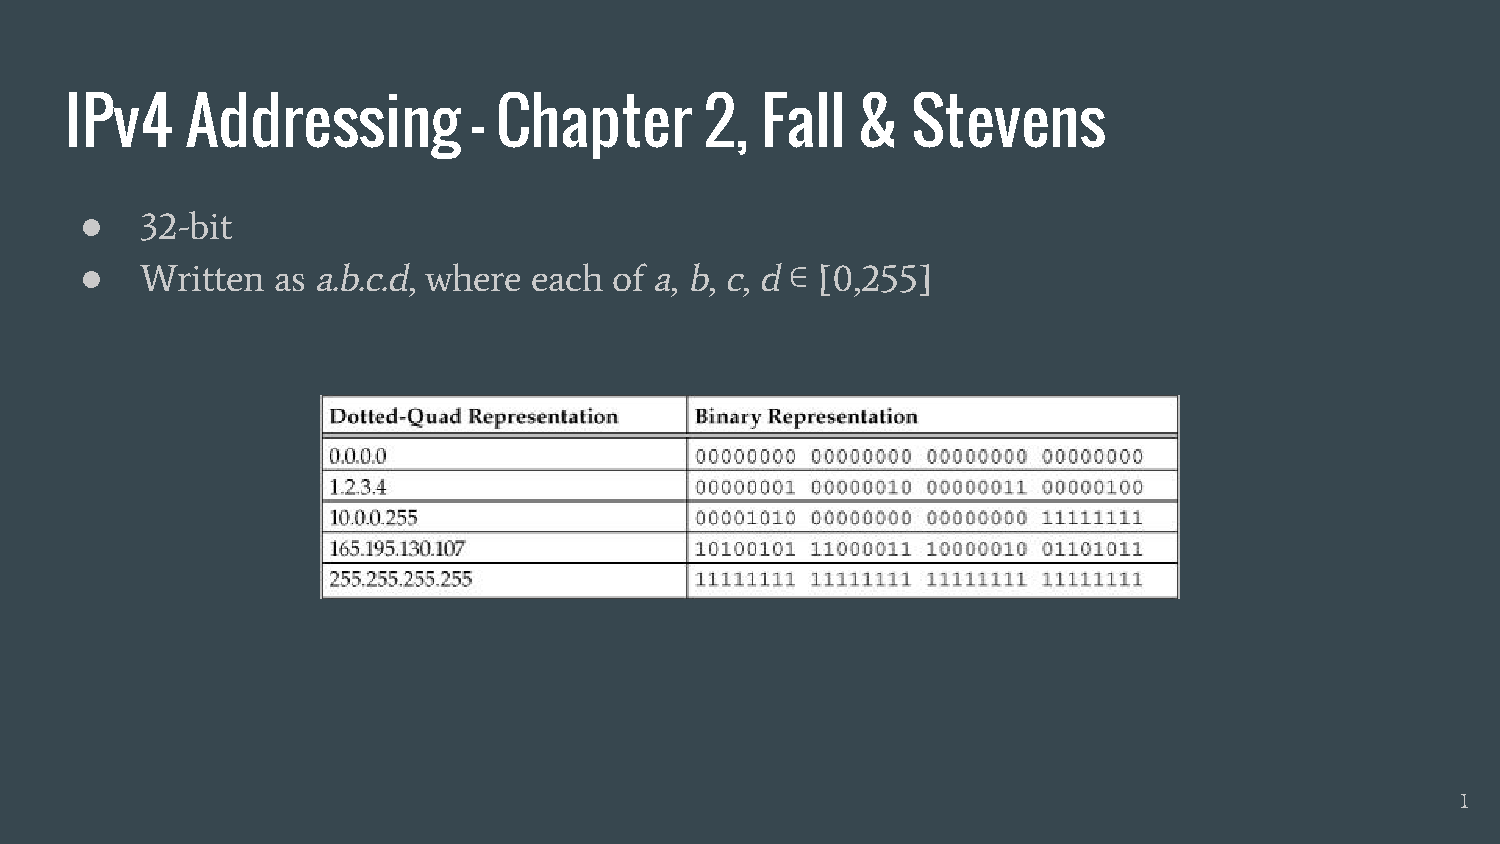
\includepdf[page=8]{slides.pdf}
A special case occurs with a mask of size 32, yes but its weird. A mask of 31 is actually thing when you have a point to point link. It results in the host ids being 0 and 1. Usually we dont use the host of 0 so that we can use it to denote the network prefix and we tend not to use 1 because it is for the ip broadcast.

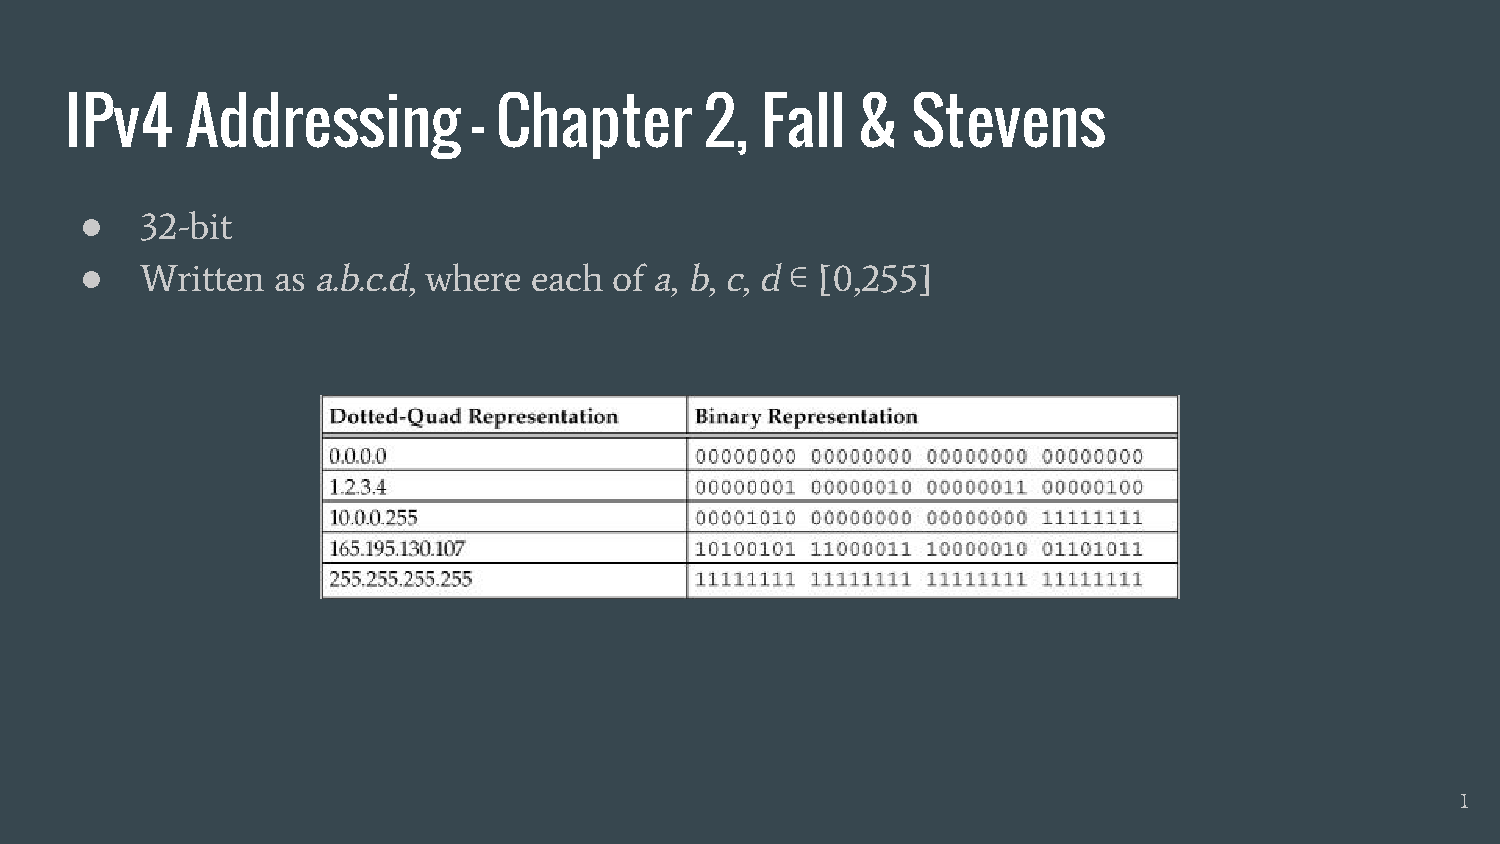
\includepdf[page=9]{slides.pdf}
The broadcast address is special. If the host id is set to all 1s it is the broadcast address. When we go to send a packet we try to send it but the routing table is going to first send it to somewhere within the network since that is how its routing table works. So your first hop is always in the same network as you. From there it goes to the site boarder router. To get out of our network you need to map an ethernet address to an ipaddress. To do this you package your destination address and broadcast it to the internet to see who knows what ethernet address corresponds to the known destination ipaddress. You can abuse the shit out of this by listening to the request for a corresponding address and just respond to it. Then you get the packet. You do need to get access to the wireless network to do this but that isnt really hard. Another thing you can do is send one packet and it goes to each of the hosts to see who knows where it goes which is a massive security issue since that packet gets cloned to hell. 

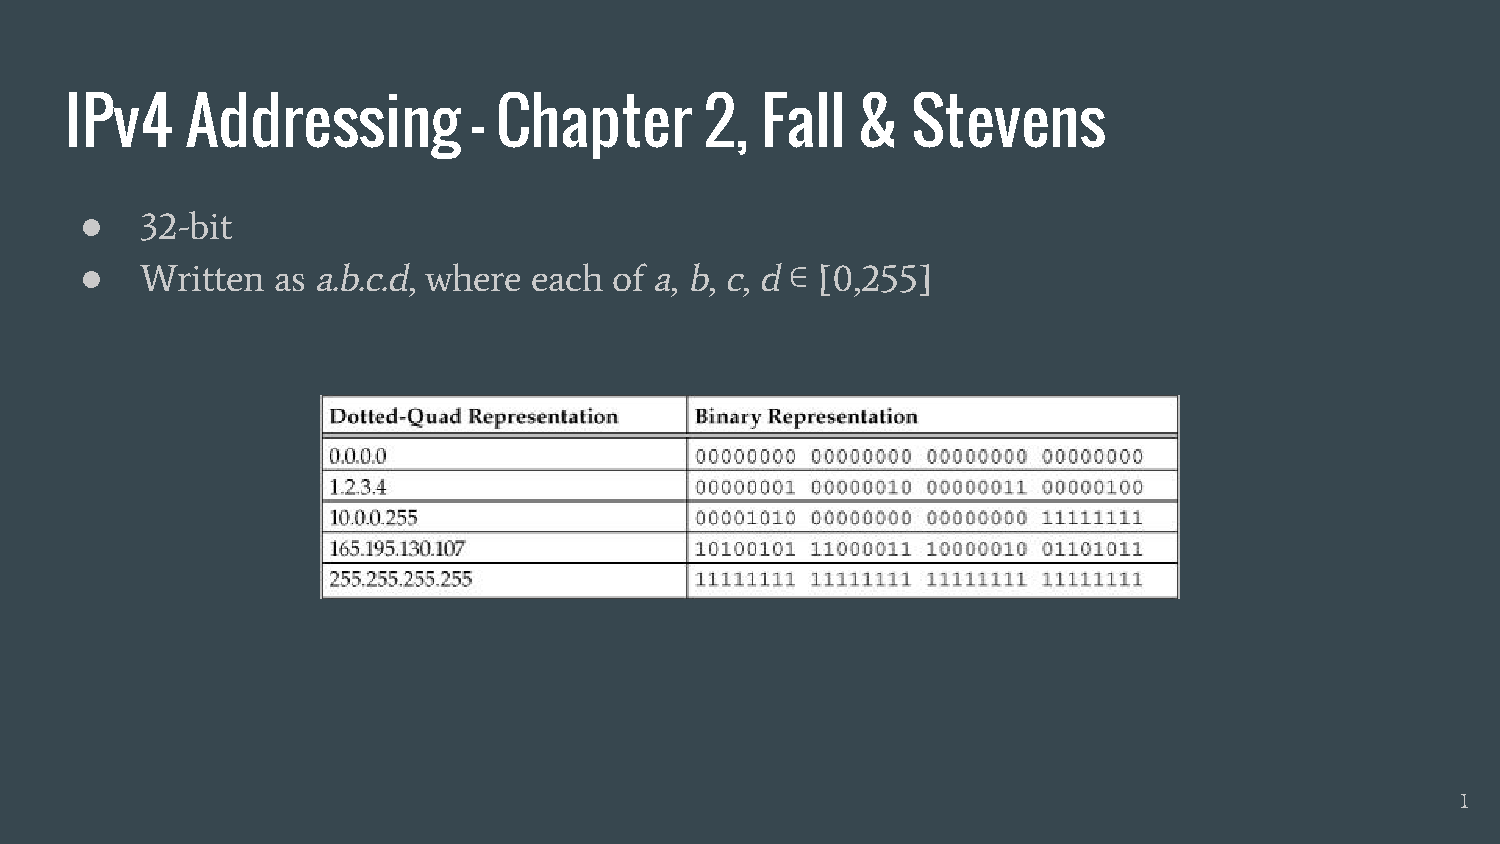
\includepdf[page=10]{slides.pdf} 
In the 90s we started running out of ipaddresses. Also all of these tables for looking up classful addresses were getting huge.

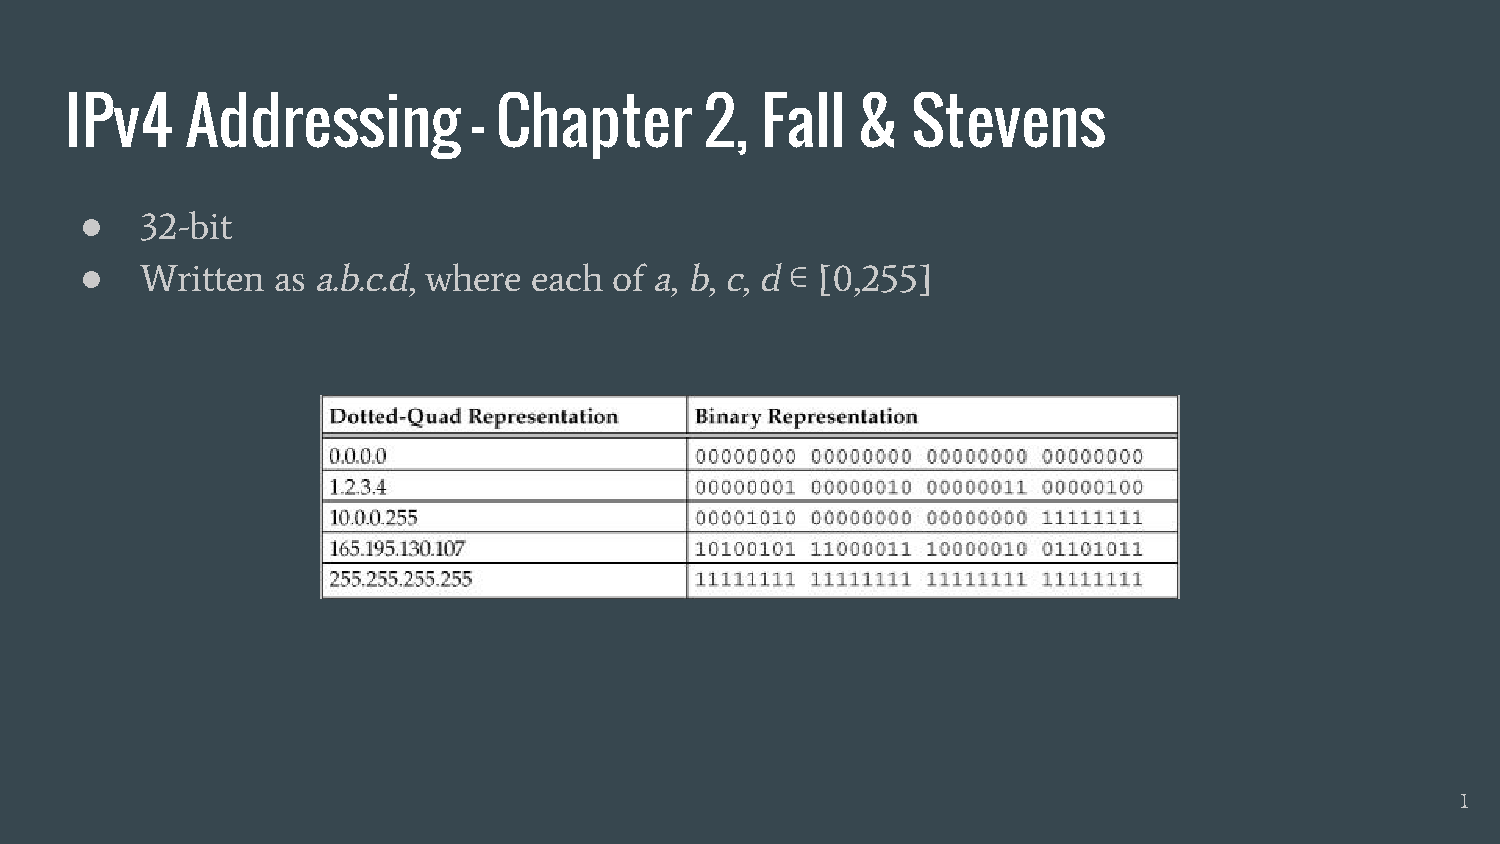
\includepdf[page=11]{slides.pdf}
A proposed solution was to forget classful addressing. You can also agregate adjacent blocks. This decresses the number of entries in the look up table, but increses the complexity of your look up algortihm.

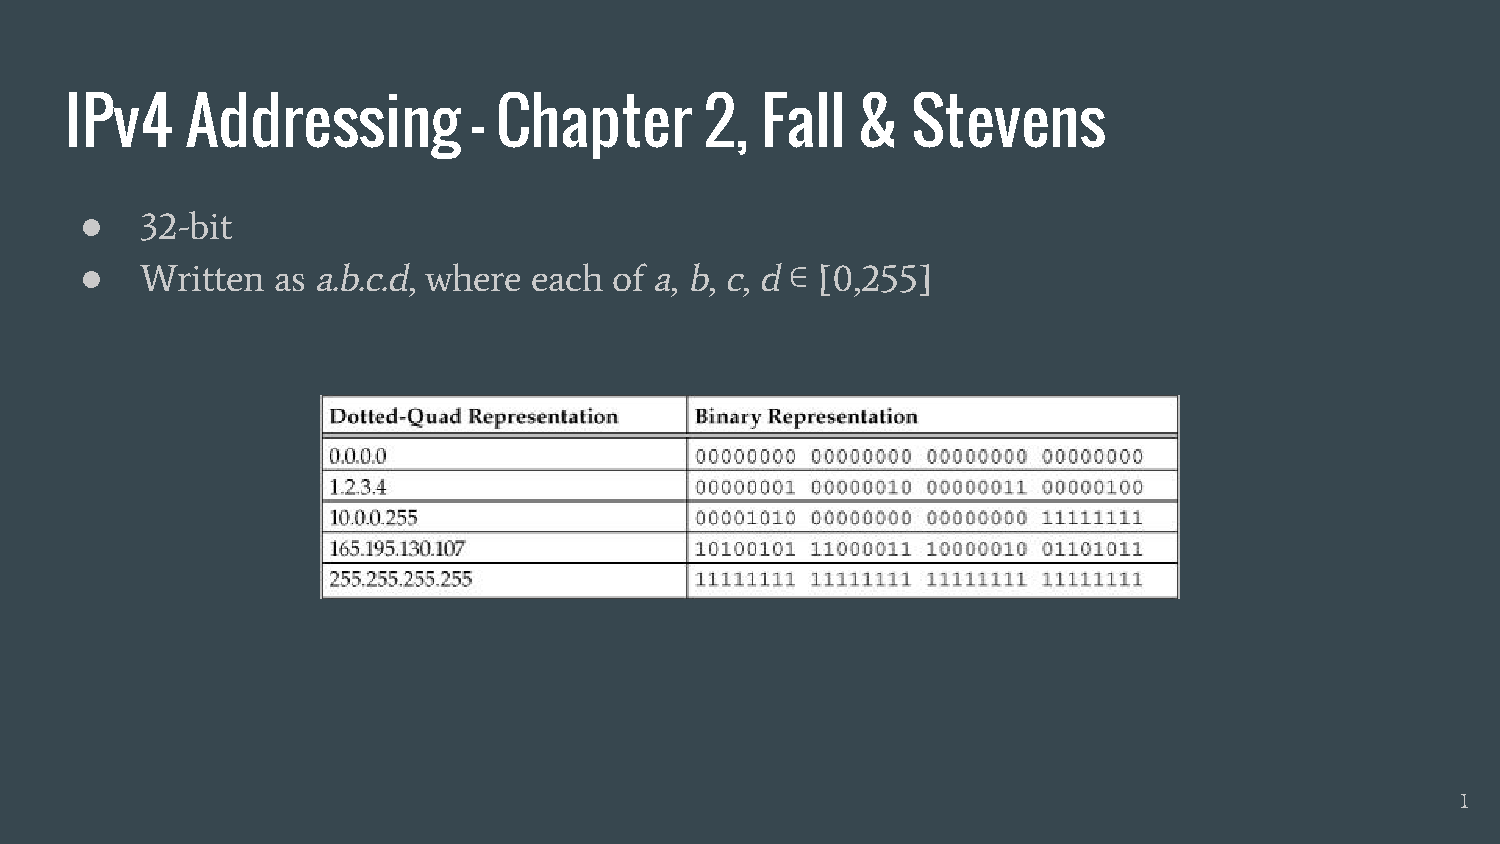
\includepdf[page=12]{slides.pdf}
When we removed the class separation it doesnt really help reduce routing table entries. 

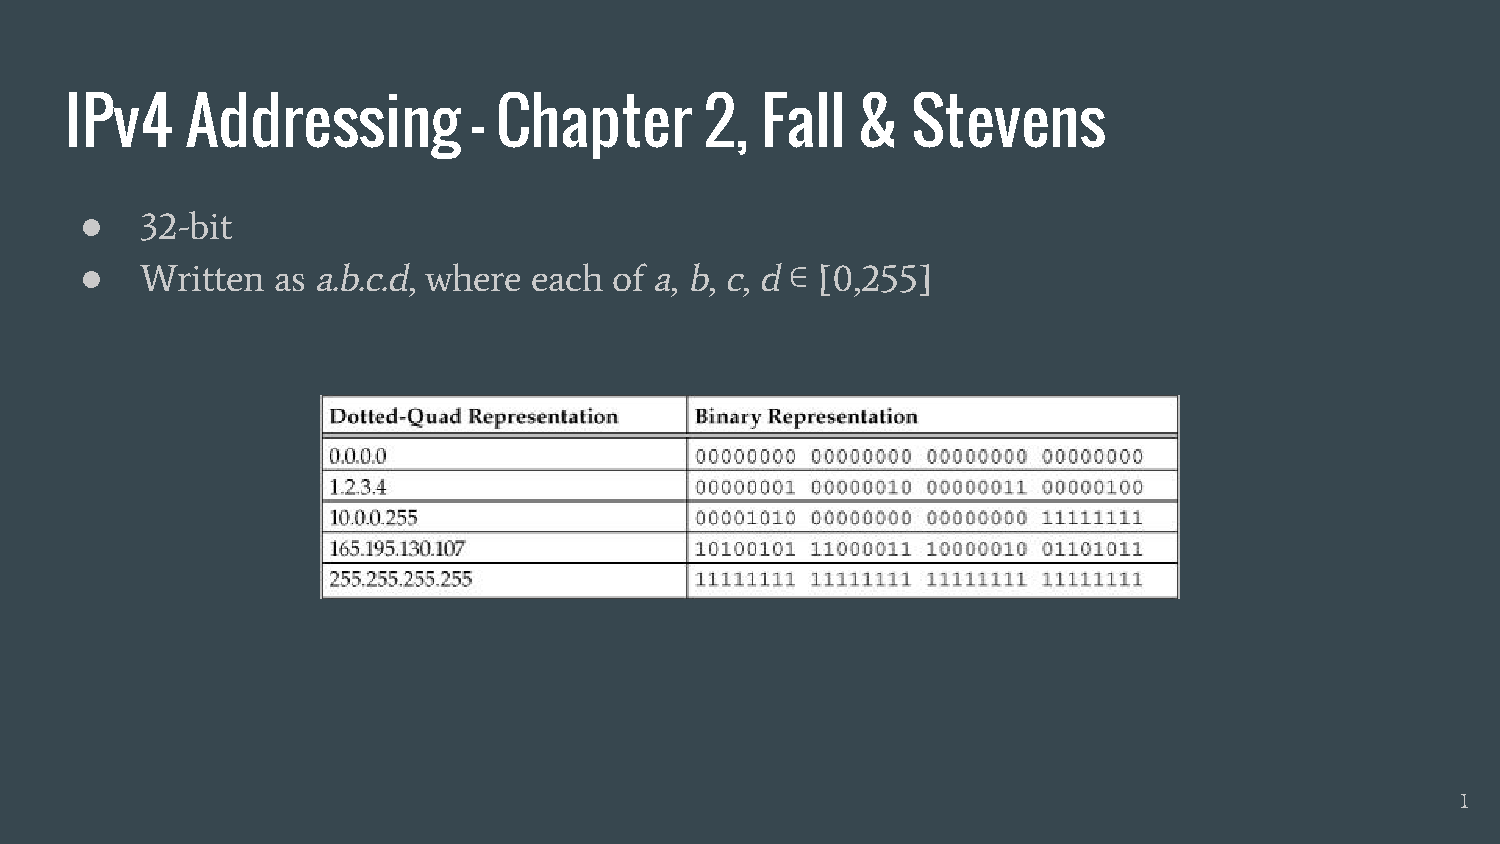
\includepdf[page=13]{slides.pdf}
If we were to make our topology a tree and leverage it we could fix a bunch of our problems. The example on the left ignores the tree topology and just hands out addresses. Because of this your router needs to keep entries for each node in the tree. If instead we leverage the tree topology only needs to know its address and its children's address. This is now in use. We tend to all get provider agregatable address. They manage these trees of addresses. 

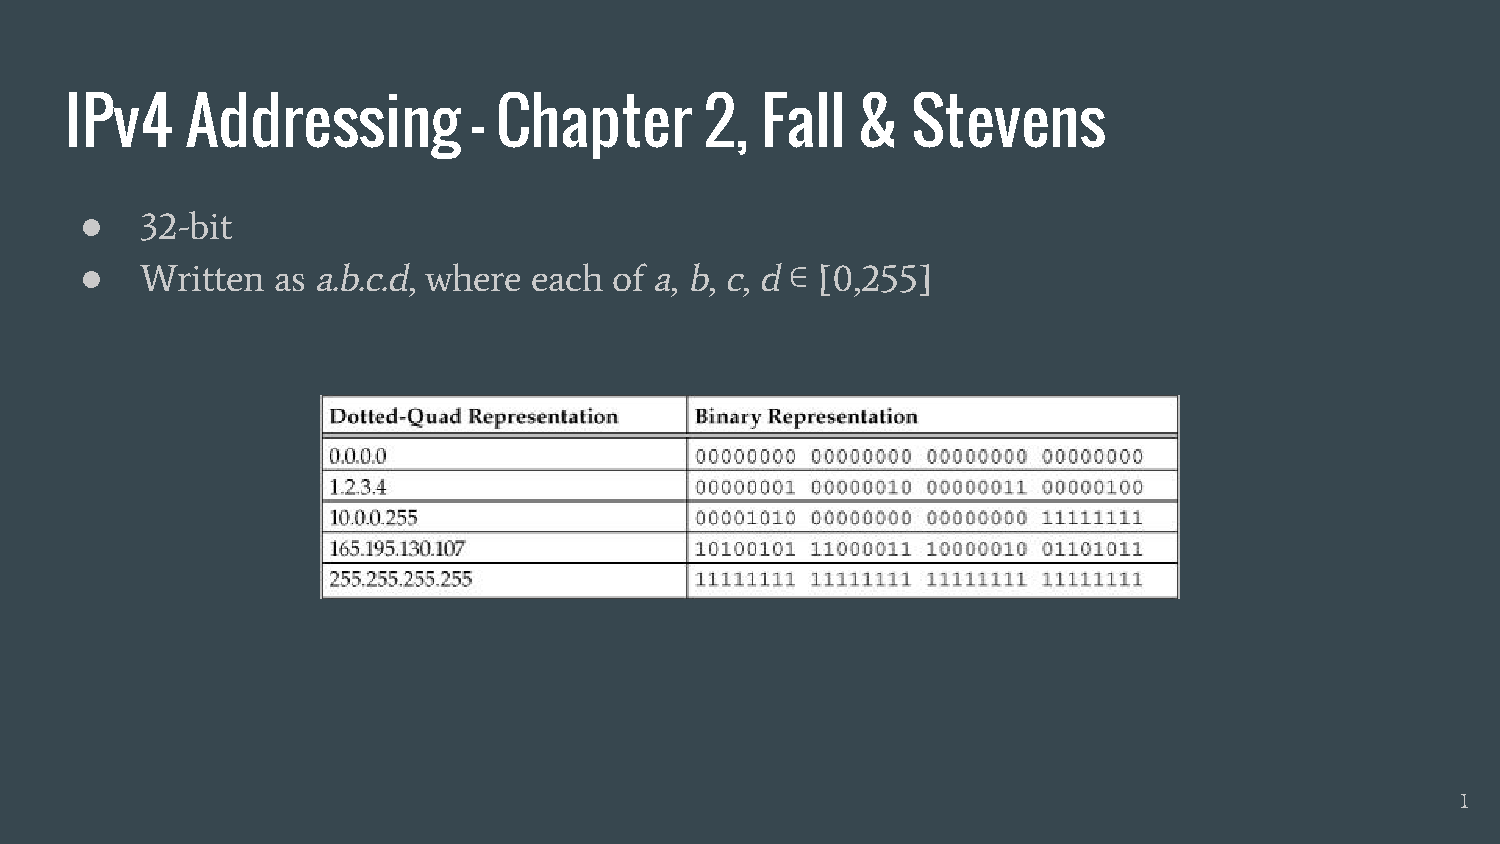
\includepdf[page=14]{slides.pdf}
In this example we can see that each address on the left have the same leading 24 bits and a mask of 26. With the first address the 25th bit is 0 and the other two have 1s so we can make its address mask shorter. We do the same for the other two and on and on to form the tree root. 

Important note: in this example more addresses are added as we go, it gets a bit confusing.

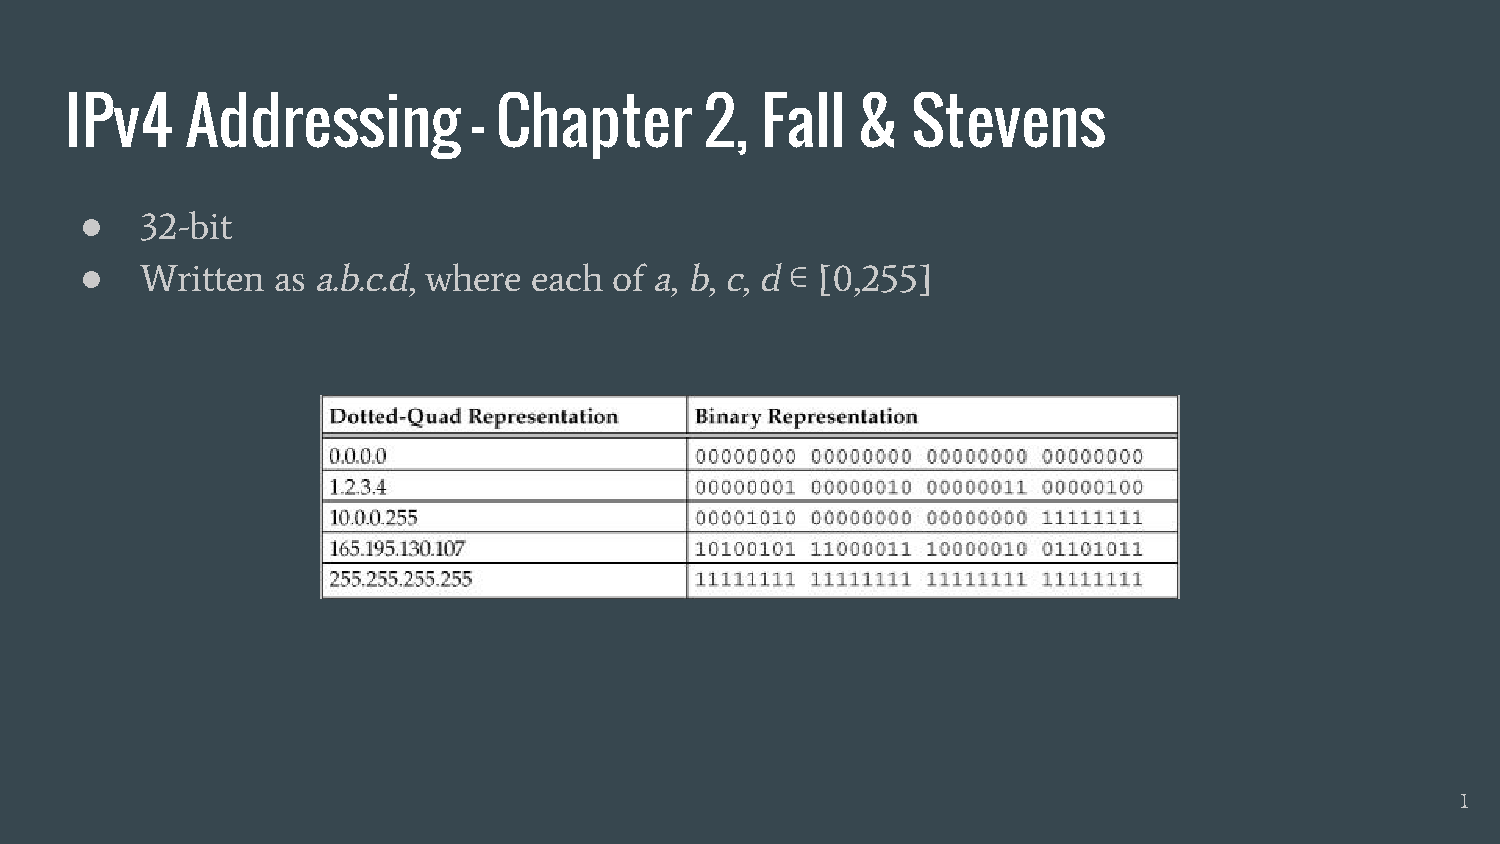
\includepdf[page=15]{slides.pdf}
There are some addresses that are special

\begin{itemize}
  \item 0.0.0.0 - source ip address
  \item 10.0.0.0, 172.16.0.0, 192.168.0.0 - private addresses
  \item 127.0.0.0 - loopback address, used to test software without sending shit out
  \item 169.254.0.0 - used for link local addresses, if you machine doesn't know what ipaddress is you just pick one in that range
  \begin{itemize}
    \item to keep people from picking the same ipaddress we use gratutious arp (address resolution protocol) chose an ip address, send out packet and see if someone has it, if so pick again
  \end{itemize}
\end{itemize}

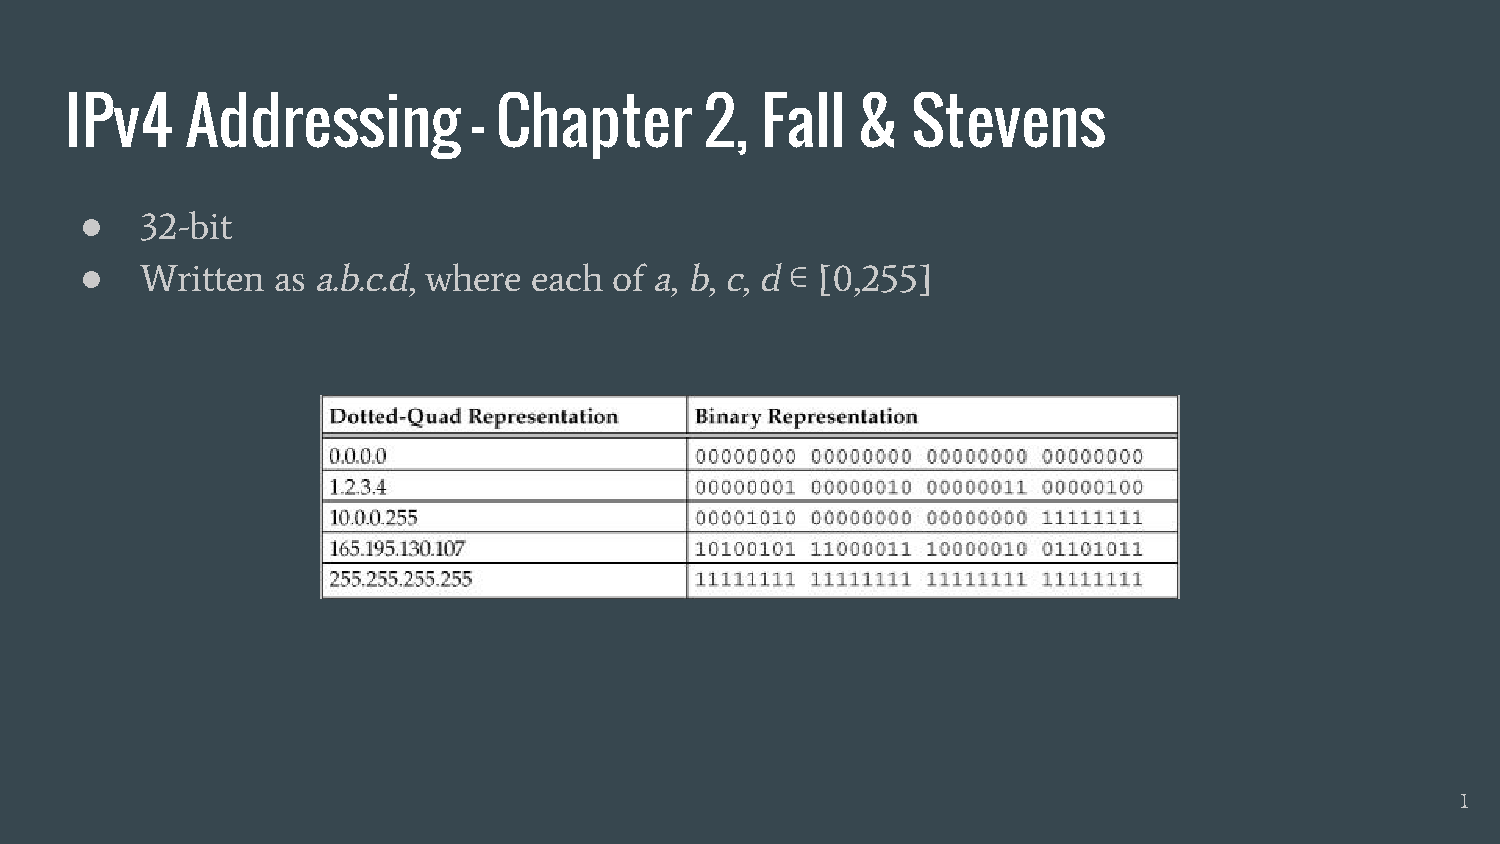
\includepdf[page=16-17]{slides.pdf}

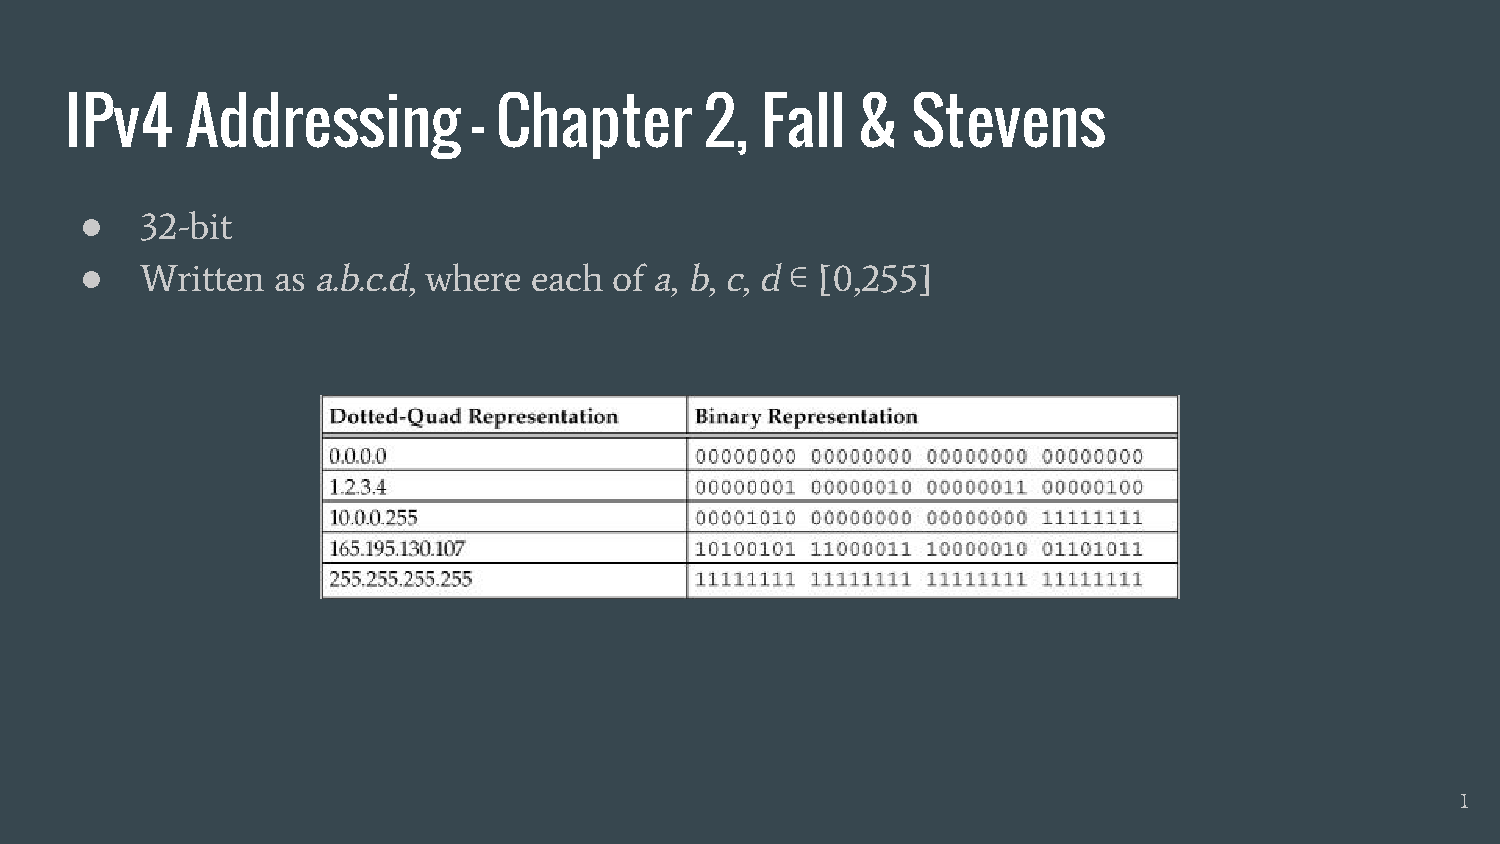
\includepdf[page=18]{slides.pdf}
We have a dematerialized zone that separates your internal network from the enterprise boarder where you can put your public facing things. 

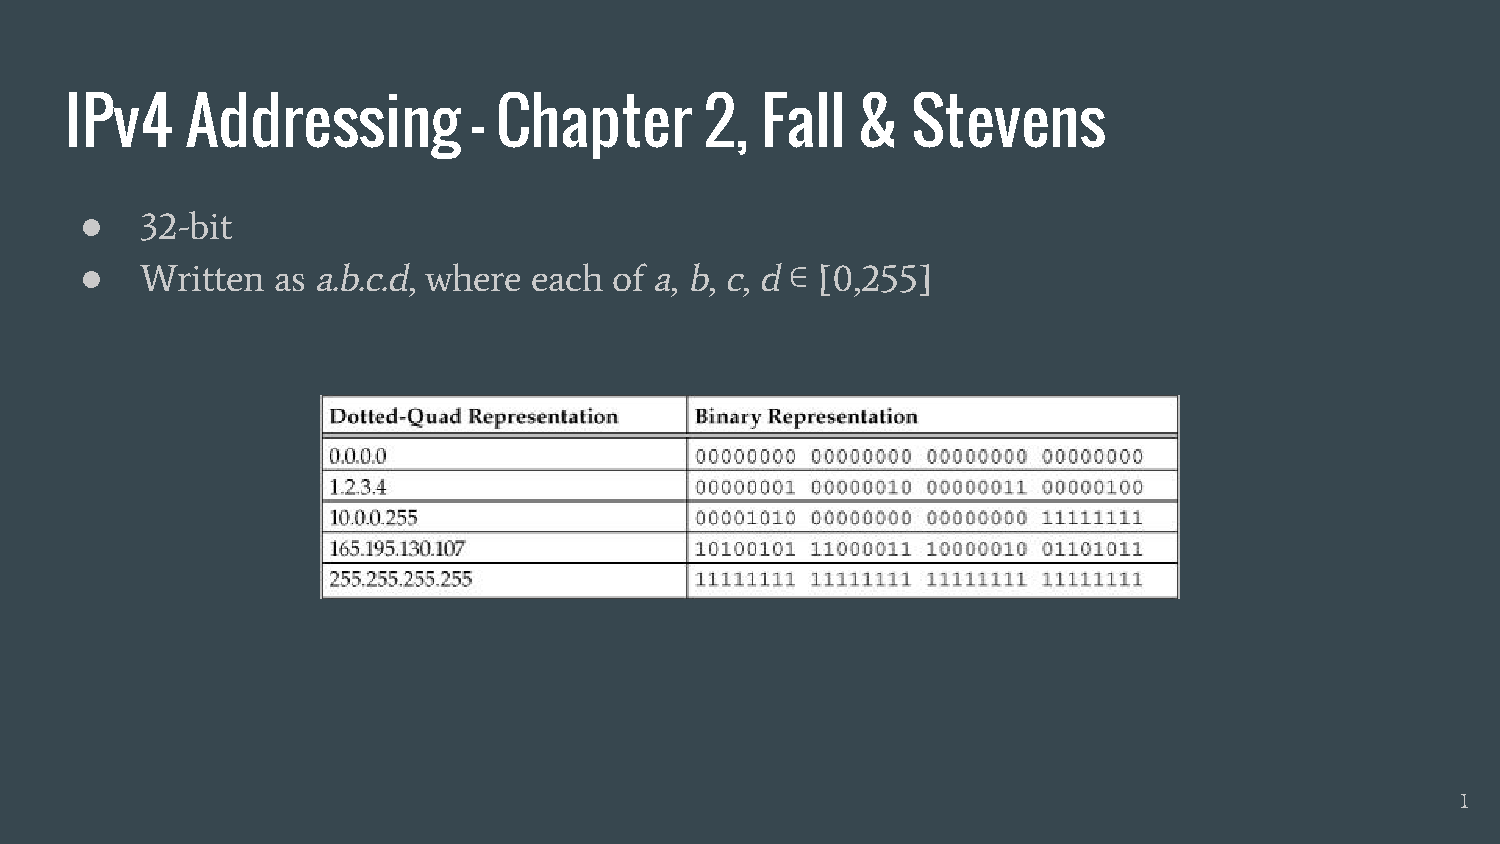
\includepdf[page=19-20]{slides.pdf}
This picture is crazy complicated in real life. When you send a packed to a network with multiple providers it applies a best fit algorithm when looking. In this example an packed with desination 12 it will actually go through isp p2 which isnt fair since isp p1 isnt getting its money worth. A solution is to not advertise that address on isp p2. Another solution is to keep them separate.



\end{document}